% !TeX document-id = {a7325568-63cb-46d1-95d6-777a45054e5a}
% !TeX TXS-program:compile = txs:///pdflatex/[--shell-escape]
\documentclass{article}
\usepackage{style}
\begin{document}
\maketitle
\tableofcontents
\section{Introducción}
En 1943 Warren S. McCulloch, un neurocientífico, y Walter Pitts, un lógico, publicaron ``A logical calculus of the ideas immanent in nervous activity'' en el ``Bulletin of Mathematical Biphysics'' 5: 115-133. En este documento, McCulloch y Pitts intentaron comprender cómo el cerebro puede producir patrones altamente complejos mediante el uso de muchas células básicas que están conectadas entre sí, estas se llaman neuronas, McCulloch  y Pitts dieron un modelo muy simplificado de una neurona en su papel,este ha hecho una contribución importante al desarrollo de redes neuronales artificiales, que modelan las características clave de las neuronas biológicas.
La célula de McCulloch-Pitts fue el primer modelo de un neurona biológica como un dispositivo de dos estados:
\begin{itemize}
	\item Apagado(0)
	\item Encendido(1)
\end{itemize}
Es la unidad esencial con la cual se construye una red neuronal artificial\\
En esta práctica usaremos un modelo similar a este ya que no tenemos bias. Usaremos aprendizaje supervisado ya que $\forall$ conjunto de valores $v$ $\exists$ un target $t$
\subsection{Modelo}
\begin{figure}[h!]
	\caption{Modelo}
	\centering
	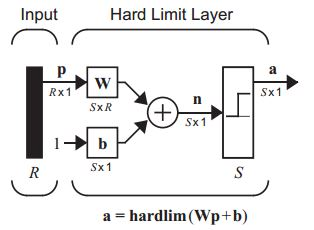
\includegraphics{model}
\end{figure}
Donde $x_1, x_2,\ldots, x_n$ son los valores de entrada, $w_1, w_2,\ldots, w_n$ son los pesos sinápticos, $\theta$ es un valor de umbral que se usa para activar la señal de entrada.\\
Matemáticamente podemos representar esta célula con las siguientes expresiones:\\
\begin{align}
	n &= \sum_{i=1}^{R}W_i*P_i
\end{align}
\begin{align}
	s &{}=\displaystyle
	\begin{cases}
		1 &\text{si } n > \theta\\
		0 &\text{en otro caso}
	\end{cases}
\end{align}
\newpage
\section{Diagrama de Flujo}
\begin{figure}[htpb]
	\centering
	\includesvg[width = 400pt, height = 400pt]{diagram}
	\caption{Diagrama de Flujo}
\end{figure}
\section{Fórmula general para las compuertas AND y OR}
Debido a que trabajamos con valores lógicos se propone que los pesos sinápticos siempre sean unos.
\subsection{AND}
La única forma de que la salida de esta sea ``1'' es que todas las entradas sean ``1's', entonces $n=w_1*p_1 + w_2*p_2 + \ldots + w_n*p_n$ se puede simplificar a $n = tam(w)$, por lo tanto, n tiene que ser mayor al umbral solo en ese caso, entonces, el umbral sería $\theta = tam(w) - 1$.\\
Explicado matemáticamente para cuando la salida de AND es 1:\\
$ p = (p_1, p_2, \ldots, p_r) = (1, 1, \ldots, 1)$\\
$ w = (w_1, w_2, \ldots, w_r) = (1, 1, \ldots, 1)$\\
$ r > 0$\\
$ n = w_1*p_1 + w_2*p2, + \ldots +w_r*p_r = tam(w)$\\
$ f(n) = 1 \rightarrow (n > \theta)$\\
$ \therefore \theta = tam(w) - 1$
\subsection{OR}
La única forma en que la salida sea '0' es que todas las entradas sean '0', entonces $ n=w_1*p_1 + w_2*p_2 + \ldots + w_n*p_n$ se puede simplificar a $ n = 0$. n tiene que ser mayor al umbral para todos los demás casos, entonces el umbral sería 0.\\
Explicado matemáticamente para cuando la salida de OR es 0:\\
$ p = (p_1, p_2, \ldots, p_r) = (0, 0, \ldots, 0)$\\
$ w = (w_1, w_2, \ldots, w_r) = (1, 1, \ldots, 1)$\\
$ r > 0$\\
$ n = w_1*p_1 + w_2*p2, + \ldots +w_r*p_r = 0$\\
$ f(n) = 0 \rightarrow (n \leq \theta)$\\
Dejando a un lado a los enteros negativos: $\theta = 0$
\section{Resultados}
\subsection{Compuerta NOT}
\begin{lstlisting}
	Ingrese la compuerta (and, or, not): not
	Ingrese el número de intentos: 1
	Ingrese el valor de los pesos sinápticos separados por espacios(e.g. 1 2 3 4): -1
	Ingrese el valor del umbral: -1
	
	model =
	
	2x2 logical array
	
	0   1
	1   0
	
	a_1 = 1 -> t_1 = 1
	a_2 = 0 -> t_2 = 0
	El aprendizaje fue exitoso
\end{lstlisting}
\subsection{Compueta AND}
\begin{lstlisting}
	Ingrese la compuerta (and, or, not): and
	Ingrese el número de intentos: 1
	Ingrese el valor de los pesos sinápticos separados por espacios(e.g. 1 2 3 4): 1 1 1 1 1
	Ingrese el valor del umbral: 4
	
	model =
	
	32x6 logical array
	0   0   0   0   0   0
	0   0   0   0   1   0
	0   0   0   1   0   0
	0   0   0   1   1   0
	0   0   1   0   0   0
	0   0   1   0   1   0
	0   0   1   1   0   0
	0   0   1   1   1   0
	0   1   0   0   0   0
	0   1   0   0   1   0
	0   1   0   1   0   0
	0   1   0   1   1   0
	0   1   1   0   0   0
	0   1   1   0   1   0
	0   1   1   1   0   0
	0   1   1   1   1   0
	1   0   0   0   0   0
	1   0   0   0   1   0
	1   0   0   1   0   0
	1   0   0   1   1   0
	1   0   1   0   0   0
	1   0   1   0   1   0
	1   0   1   1   0   0
	1   0   1   1   1   0
	1   1   0   0   0   0
	1   1   0   0   1   0
	1   1   0   1   0   0
	1   1   0   1   1   0
	1   1   1   0   0   0
	1   1   1   0   1   0
	1   1   1   1   0   0
	1   1   1   1   1   1
	
	a_1 = 0 -> t_1 = 0
	a_2 = 0 -> t_2 = 0
	a_3 = 0 -> t_3 = 0
	a_4 = 0 -> t_4 = 0
	a_5 = 0 -> t_5 = 0
	a_6 = 0 -> t_6 = 0
	a_7 = 0 -> t_7 = 0
	a_8 = 0 -> t_8 = 0
	a_9 = 0 -> t_9 = 0
	a_10 = 0 -> t_10 = 0
	a_11 = 0 -> t_11 = 0
	a_12 = 0 -> t_12 = 0
	a_13 = 0 -> t_13 = 0
	a_14 = 0 -> t_14 = 0
	a_15 = 0 -> t_15 = 0
	a_16 = 0 -> t_16 = 0
	a_17 = 0 -> t_17 = 0
	a_18 = 0 -> t_18 = 0
	a_19 = 0 -> t_19 = 0
	a_20 = 0 -> t_20 = 0
	a_21 = 0 -> t_21 = 0
	a_22 = 0 -> t_22 = 0
	a_23 = 0 -> t_23 = 0
	a_24 = 0 -> t_24 = 0
	a_25 = 0 -> t_25 = 0
	a_26 = 0 -> t_26 = 0
	a_27 = 0 -> t_27 = 0
	a_28 = 0 -> t_28 = 0
	a_29 = 0 -> t_29 = 0
	a_30 = 0 -> t_30 = 0
	a_31 = 0 -> t_31 = 0
	a_32 = 1 -> t_32 = 1
	El aprendizaje fue exitoso
\end{lstlisting}
\subsection{Compuerta OR}
\begin{lstlisting}
	Ingrese la compuerta (and, or, not): or
	Ingrese el número de intentos: 1
	Ingrese el valor de los pesos sinápticos separados por espacios(e.g. 1 2 3 4): 1 1 1 1 1
	Ingrese el valor del umbral: 0
	
	model =
	
	32x6 logical array
	
	0   0   0   0   0   0
	0   0   0   0   1   1
	0   0   0   1   0   1
	0   0   0   1   1   1
	0   0   1   0   0   1
	0   0   1   0   1   1
	0   0   1   1   0   1
	0   0   1   1   1   1
	0   1   0   0   0   1
	0   1   0   0   1   1
	0   1   0   1   0   1
	0   1   0   1   1   1
	0   1   1   0   0   1
	0   1   1   0   1   1
	0   1   1   1   0   1
	0   1   1   1   1   1
	1   0   0   0   0   1
	1   0   0   0   1   1
	1   0   0   1   0   1
	1   0   0   1   1   1
	1   0   1   0   0   1
	1   0   1   0   1   1
	1   0   1   1   0   1
	1   0   1   1   1   1
	1   1   0   0   0   1
	1   1   0   0   1   1
	1   1   0   1   0   1
	1   1   0   1   1   1
	1   1   1   0   0   1
	1   1   1   0   1   1
	1   1   1   1   0   1
	1   1   1   1   1   1
	
	a_1 = 0 -> t_1 = 0
	a_2 = 1 -> t_2 = 1
	a_3 = 1 -> t_3 = 1
	a_4 = 1 -> t_4 = 1
	a_5 = 1 -> t_5 = 1
	a_6 = 1 -> t_6 = 1
	a_7 = 1 -> t_7 = 1
	a_8 = 1 -> t_8 = 1
	a_9 = 1 -> t_9 = 1
	a_10 = 1 -> t_10 = 1
	a_11 = 1 -> t_11 = 1
	a_12 = 1 -> t_12 = 1
	a_13 = 1 -> t_13 = 1
	a_14 = 1 -> t_14 = 1
	a_15 = 1 -> t_15 = 1
	a_16 = 1 -> t_16 = 1
	a_17 = 1 -> t_17 = 1
	a_18 = 1 -> t_18 = 1
	a_19 = 1 -> t_19 = 1
	a_20 = 1 -> t_20 = 1
	a_21 = 1 -> t_21 = 1
	a_22 = 1 -> t_22 = 1
	a_23 = 1 -> t_23 = 1
	a_24 = 1 -> t_24 = 1
	a_25 = 1 -> t_25 = 1
	a_26 = 1 -> t_26 = 1
	a_27 = 1 -> t_27 = 1
	a_28 = 1 -> t_28 = 1
	a_29 = 1 -> t_29 = 1
	a_30 = 1 -> t_30 = 1
	a_31 = 1 -> t_31 = 1
	a_32 = 1 -> t_32 = 1
	El aprendizaje fue exitoso
\end{lstlisting}
\section{Discusión de Resultados}
Para cada uno de los resultados se muestra:
\begin{enumerate}
	\item Los datos ingresados por el usuario
	\item La tabla de verdad que contiene las entradas y su target de la siguiente manera:
	\begin{lstlisting}[mathescape=true]
		model = 
		$P_{11}$ $P_{12}$ $\ldots$ $P_{1n}$ $target_1$
		$P_{21}$ $P_{22}$ $\ldots$ $P_{2n}$ $target_2$
		$\dots\dots\dots\dots\dots\dots\dots\dots\dots$
		$P_{m1}$ $P_{m2}$ $\ldots$ $P_{mn}$ $target_m$
	\end{lstlisting}
	Donde $n$ es el tamaño del vector de entradas y $m = 2^n$
	\item Si la neurona está activada con base en el índice del modelo y el target
	\item Si el aprendizaje fue existoso o no
\end{enumerate}
En la tabla de verdad los target se calcularon mediante la aplicación de la operación correspondiente (AND, OR o NOT), por ejemplo, para la AND se puede ver que el target es 1 solo cuando todas las entradas son 1. \\
El tamaño de las entradas se calculan con base en los pesos que ingresó el usuario, por ejemplo, si el usuario ingresa los pesos: 1 1 1 1, se generará una tabla de $2^4$ filas y 5 columnas, donde las primeras 4 son las entradas y la última su target.\\
En cada caso se muestra que el aprendizaje fue exitoso y se puede comprobar con la salida del programa para cada índice.
\section{Conclusiones}
La célula de McCulloch-Pitts fue una muy importante aportación para las Ciencias de la Computación ya que fue la base para resolver problemas que no tenían solución, con base en la aportación se desarrollaron diferentes arquitecturas, cada una de ellas contiene como su unidad a la célula de McCulloch-Pitts. En esta práctica logré comprender el funcionamiento individual de la célula y su comportamiento como las tres compuertas lógicas básicas, al igual que aprendí a usar la plataforma MATLAB, no hay duda de que es una gran herramienta cualquier Académico.
\section{Referencias}
D. Michie, D.J. Spiegelhalter, C.C. Taylor (eds). Machine Learning, Neural and Statistical Classification, 1994.\\
\url{http://www.mind.ilstu.edu/curriculum/modOverview.php?modGUI=212}
\section{Apéndice}
\begin{lstlisting}[
style=Matlab-editor,
basicstyle=\mlttfamily,
escapechar=`,
caption={Código},
]
% Datos proporcionados por el usuario
gate = input('Ingrese la compuerta (and, or, not): ', 's');
tries = input('Ingrese el número de intentos: ');
for i = 1:tries
	syn_prompt = 'Ingrese el valor de los pesos sinápticos separados por espacios(e.g. 1 2 3 4): ';
	w = str2num(strip(input(syn_prompt, 's')));
	theta = input('Ingrese el valor del umbral: ');
	if (gate == "not" && size(w, 2) > 1)
		fprintf("Error, la compuerta NOT es de una sola entrada");
	else
		% Generación de la tabla de entradas y targets
		model = logicalModel(size(w, 2), gate)
		error = false;
		% Época
		for i = 1:size(model, 1)
			row = model(i, :);
			% Obtención de n
			n = sum(row(1:end-1).*w);
			% Obtención de a
			if(n > theta); a_n = 1; else; a_n=0; end
			% Comparación de a con el target
			fprintf("a_%i = %i -> t_%i = %i\n", i, a_n, i, row(end));
			if(a_n ~= row(end)); error = true; break; end
		end
		if(~error); fprintf("El aprendizaje fue exitoso\n");break; else 
		fprintf("El aprendizaje no fue exitoso\n"); end
	end
end


function [table] = logicalModel(i, gate)
% logicalModel(I, gate) returns a matrix representing a truth table and
% the last column represents the oupot base on all the previous columns
% based on the (gate) parameter
% INPUT: (I) shall be an integer >= 1
% INPUT: (gate) shall be 'and' or 'or'
% OUTPUT: logicalModel is a binary matrix of size [2^I,I + 1]
% Heavily inspired in Paul Metcalf's CONDVECTS
% Acknowledgements: Paul Metcalf

g = 2;
i2 = 2^i;
table = false(i2,i + 1);
for m = 1 : 1 : i
	m2 = 2^m;
	m3 = (m2/2)-1;
	i3 = i-m+1;
	for g = g : m2 : i2
		for k = 0 : 1 : m3
			table(g+k,i3) = true;
		end
	end
	g = m2+1;
end
	if (gate == "and")
		for row_index = 1:size(table, 1)
			row = table(row_index,:);
			res = row(1);     
			for e_index = 1:size(row, 2)-1
				res = res & row(e_index);
			end
			table(row_index, end) = res; 
		end  
	elseif (gate == "or")
		for row_index = 1:size(table, 1)
		row = table(row_index,:);
			res = row(1);     
			for e_index = 1:size(row, 2)-1
				res = res | row(e_index);
			end
			table(row_index, end) = res; 
		end 
	elseif (gate == "not")
		for row_index = 1:size(table, 1)
			row = table(row_index,:);
			res = ~row(1);     
			table(row_index, end) = res; 
		end
	end  
end
\end{lstlisting}
\end{document}